\documentclass{beamer}
\usepackage{cancel}
\usepackage{listings}
\title{23MAT112 End-Sem Project \\ Discrete Fourier Analysis And The Fast Fourier Transform}
\author{Group 2}
\institute{Amrita Vishwa Vidyapeetham}
\date{23rd May 2024}
\usetheme{Hannover}

% Berkeley, Hannover

\begin{document}
\maketitle
\begin{frame}
\frametitle{Overview}
\tableofcontents
\end{frame}
\section{Discrete Fourier Analysis}
\begin{frame}
	\frametitle{The Motivation}
	The Fourier Transform is an algorithm that has made many parts of modern-day life possible.
\end{frame}
	\subsection{Background}
\begin{frame}
		\frametitle{Sampling}
For $n$ samples, $x_j$ is one such sample point between the interval $[a,b]$, such that,
		\begin{align*}
	&x_j = a + jh, \ j = 0, \dots, n, & \text{where} \ h = \frac{b-a}{n} \\
		\end{align*}
		\pause
		We will use the ``standard" interval $[0,2\pi]$ which means,
		\[
				x_0 = 0, x_1 = \frac{2\pi}{n}, x_2 = \frac{4\pi}{n}, x_j = \frac{2j\pi}{n}, x_{n-1} = \frac{2(n-1)\pi}{n}
		\]
		\pause
		\begin{block}{Remark}
			Functions defined on other intervals can simply be rescaled to fit the interval $[0,2\pi]$
		\end{block}
\end{frame}
\begin{frame}
\frametitle{An Important Consequence}
We will now write the sampled output at a given sample $x_j$ as $f_j$, in other words $f_j = f(x_j)$.
\linebreak
Take the function,
\[
	f(x) = e^{inx}
\]
Let's take $n$ equally spaced samples, $x_j = \frac{2\pi j }{n}$.
\[
	f_j = f(\frac{2j \pi}{n}) \pause = exp(in \frac{2j\pi}{n}) \pause = e^{2j\pi i} \pause = 1
\]
For all values of $x_j$, $f_j = 1$
\pause

\textbf{This means that taking $n$ equally spaced samples cannot give back the periodic function of frequency $n$}
\end{frame}
\begin{frame}
	\frametitle{An Important Consequence}
	For $n$ equally spaced samples,
	\[
		e^{i(k+n)x} = e^{ikx}
	\]
	\pause
	And more importantly, we can convert negative frequencies to positive frequencies,
	\[
		e^{-ikx} = e^{i(n-k)x} 
	\]
	\pause
	For $n$ samples, the discrete Fourier representation only needs $n$ complex exponentials.(More on that later.)
\end{frame}
\begin{frame}
	\frametitle{Discrete Fourier Representation}
	For $n$ samples, the Fourier representation is,
	\[
			f(x) \sim p(x) = c_0 + c_1 e^{ix} + c_2 e^{2ix} + \cdots + c_{n-1}e^{(n-1)ix}
	\]
	\pause
	\begin{block}{Note}
			If $f(x)$ is real then $p(x)$ is real, at the sampled points, but the function could be complex in between. The imaginary component of the function is removed and $p(x)$ is treated as the interpolating trigonometric polynomial of the function $f(x)$. But, the representation is still retained for convenience.

	\end{block}
\end{frame}
\begin{frame}
	\frametitle{Complex Vectors}
	For $f_0$,
	\[
		p(x_0) = c_0 + c_1 e^{ix_0} + c_2 e^{2ix_0} + \cdots + c_{n-1}e^{(n-1)ix_0}
	\]
	\pause
	For $f_j$,
	\[
		p(x_j) = c_0 + c_1 e^{ix_j} + c_2 e^{2ix_j} + \cdots + c_{n-1}e^{(n-1)ix_j}
	\]
	\pause
	We define a complex vector $\vec{\omega}$ to find all values of $f_j$,
	\begin{align*}
		\vec{\omega_k} &= [e^{i k x_0},e^{ik x_1},\cdots,e^{ik x_{n-1}}]^T \\
		\vec{\omega_k} &= [1,e^{i k \frac{2\pi}{n}},e^{ik \frac{4\pi}{n}},\cdots,e^{ik \frac{2\pi(n-1)}{n}}]^T \\
	\end{align*}
	\pause
	Now we can write for the sample vector $\vec{f}$ with components $f_j$
	\[
		\vec{f} = c_0 \vec{\omega_0} + c_1 \vec{\omega_1} + \cdots + c_{n-1}\omega_{n-1}
	\]
\end{frame}
\begin{frame}
	\frametitle{Inner Product For Vectors in $\mathbb{C}^n$}
	\[
			\langle f,g \rangle = \frac{1}{n} \sum_{j = 0}^{n-1} f_j \overline{g_j} = \frac{1}{n} f(x_j) \overline{g(x_j)}
	\]
	Where $\overline{g(x_j)}$ is the complex conjugate of $g(x_j)$
	\begin{block}{Remark}
		This is a rescaled version of the standard Hermitian dot product between complex vectors
	\end{block}
\end{frame}
\begin{frame}
	\begin{theorem}
			The sampled exponential vectors $\omega_0, \cdots , \omega_{n-1}$ form an orthogonal basis in $\mathbb{C}^n$ with respect to the inner product,
	\[
		\langle f,g \rangle = \frac{1}{n} \sum_{j=0}^{n-1} f_j \overline{g_j}
	\]
	\end{theorem}
	To prove this, an understanding of nth roots of unity is required.
\end{frame}
\subsection{Nth Roots Of Unity And Orthonormality}
\begin{frame}
	\frametitle{Nth Roots Of Unity}
	\begin{definition}
	A number $z \in \mathbb{C}$ satisfying the equation, where $n \in Z^+$,
	\[
	z^n = 1
	\]
	\end{definition}
	\pause
	We define,
	\[
		\zeta_n = e^{2\pi i /n}
	\]
	Where,
	\[
		\zeta_n^n = e^{(2 \pi i / n)n} = 1
	\]
	\pause
	Which means that $\zeta_n = \sqrt[n]{1}$.
\end{frame}
\begin{frame}
	\frametitle{Nth Roots Of Unity}	
	Any $k^{th}$ power of $\zeta_n$ is also an $n^{th}$ root of unity
	\[
	(z^k)^n = (z^n)^k = 1^k = 1
\]
\pause
So for the polynomial $z^n - 1$,
\[
		z^{n}-1 = (z-1)(z -  \zeta_n)(z-\zeta_n^2)\cdots(z - \zeta_n^{n-1}) 
\]
\end{frame}
\begin{frame}
\frametitle{Proving The Theorem}
		Take $\zeta_n^k = e^{2\pi k i/n}$, this means that $\zeta^n_n = 1$, and there are n equally spaced such complex numbers, between $\zeta_1$ and $\zeta_n$.
	\begin{align*}
		z^{n}-1 &= (z-1)(z -  \zeta_n)(z-\zeta_n^2)\cdots(z - \zeta_n^{n-1}) \\
		z^n-1 &= (z-1)(1 + z + z^2 + \cdots + z^{n-1}) 
	\end{align*}
	\pause
	We equate the two to get,
	\begin{align*}
	(z-1)(1 + z + \cdots + z^{n-1})  &= (z-1)(z -  \zeta_n)\cdots(z - \zeta_n^{n-1}) \\
	1 + z + \cdots + z^{n-1}  &= (z -  \zeta_n)\cdots(z - \zeta_n^{n-1}) \\
		1 + \zeta_n^k + \zeta_n^{2k} + \cdots + \zeta_n^{(n-1) k} &= \{n,k = 0 \text{ and } 0, 0 < k < n \} \\
	\end{align*}
\pause	
This extends to all integers $k$, If $k$ is a multiple of $n$, then the sum gives $n$, while giving 0 otherwise.
\end{frame}
\begin{frame}
	\frametitle{Proving The Theorem}
	Writing the sampled exponential vectors in terms of the $n^{th}$ roots of unity,

\[
	\omega_k = (1, \zeta_n^k, \zeta_n^{2k},\zeta_n^{3k}, \cdots, \zeta_n^{(n-1)k})^T
\]
\pause

We get, 
\begin{align*}
	\langle	\omega_k, \omega_l \rangle &= \frac{1}{n} \sum_{j=0}^{n-1} \zeta_{n}^{jk} \overline{\zeta_{n}^{jl}} \\
	&= \frac{1}{n} \sum_{j=0}^{n-1} \zeta_n^{j(k-l)} = \{1, k = l \text{ and } 0, k \neq l\}
\end{align*}
\end{frame}
\subsection{Computing The Coefficients}
\begin{frame}
	\frametitle{Refresher On Orthogonal Bases}
	The properties of an orthonormal basis allows us to isolate any given component $v_i$ of the vector $\vec{v}$ by simply performing the inner product of $\vec{q_i}$ with the vector $\vec{v}$
$	(\vec{q_i}\cdot \vec{q_j} = 0, \vec{q_i} \cdot \vec{q_i} = 1)$
\begin{align*}
	\vec{q_i}^T\vec{v} &= \vec{q_i}^T v_1 \vec{q_1} + \vec{q_i}^T v_2 \vec{q_2} + \cdots + \vec{q_i}^T v_i \vec{q_i} + \cdots + \vec{q_i}^T v_n \vec{q_n} \\
	\vec{q_i}^T \vec{v} &= v_i 
\end{align*}
\end{frame}
\begin{frame}
	\frametitle{Isolating Fourier Coefficients}
	We apply the inner product of $\vec{f}$ with $\omega_k$ to get the coefficient $c_k$
	\[
	c_k = \langle f, \omega_k \rangle = \frac{1}{n} \sum_{j=0}^{n-1} f_j \overline{e^{ikx_j}} \pause =  \frac{1}{n} \sum_{j=0}^{n-1} \zeta_n^{-jk} f_j
\]
\end{frame}
\begin{frame}
	\begin{definition}
The passage from a signal to its Fourier coefficients is known as The \textbf{Discrete Fourier Transform}
\end{definition}


\begin{definition}
The reconstruction of a signal from its Fourier coefficients is known as the \textbf{Inverse Discrete Fourier Transform}
\end{definition}
\end{frame}
\subsection{Matrix Form}
\begin{frame}
	\frametitle{Matrix Form}
For a given Fourier coefficient,

\[
	{c}_k = \frac{1}{n}\sum_{j=0}^{n-1} f_j \zeta_n^{-jk}
\]

So we can construct a Vandermonde matrix $F_n$ where a given term $a_{ij} = \zeta_n^{ij}$, where $i,j = 0, \cdots, {n-1}$
\[
	\begin{bmatrix}
		c_{0} \\
		c_{1} \\
		c_{2} \\
		\vdots \\
		c_{n-1} 
	\end{bmatrix}
	=
	\begin{bmatrix}
		1 & 1 & 1 & \cdots & 1 \\
		1 & \zeta_n & \zeta_n^2 & \cdots & \zeta_n^{n-1} \\
		1 & \zeta_n^2 & \zeta_n^4 & \cdots & \zeta_n^{2(n-1)} \\
		\vdots & \vdots & \vdots & \ddots & \vdots \\
		1 & \zeta_n^{n-1} & \zeta_n^{2(n-1)} & \cdots & \zeta_n^{(n-1)^2}
	\end{bmatrix}
	\begin{bmatrix}
		f_0 \\
		f_1 \\
		f_2 \\
		\vdots \\
		f_{n-1}
	\end{bmatrix}
\]
\end{frame}
\section{Fast Fourier Transform}
\begin{frame}
	\frametitle{Fast Fourier Transform}
	\begin{enumerate}
		\item<1-> The Discrete Fourier Transform has a time complexity $O(n^2)$
			\item<2-> James Cooley and John Tukey discovered a much more efficient method to compute the DFT, in the 1960s
			\item<3->This new algorithm has a time complexity $O(n\log{n})$
	\end{enumerate}
	
\end{frame}
\begin{frame}
	\frametitle{The Fast Fourier Transform}	
	The key idea is, for $n$ samples, if $n$ is even, There exists an $m$ such that $n = 2m$,
	\begin{itemize}
		\item<1-> Split the signal into halves, one set of even samples and one set of odd samples each with $m$ samples
		\item<2-> $\zeta_n^2 = \zeta_m$
		\item<3-> Split m into halves, one set of even samples and one set of odd samples
		\item<3-> Repeat until number of function samples cannot be halved.
	\end{itemize}
	\pause
	Clearly, it is best for functions where $n$ is be a power of 2.

\end{frame}
\begin{frame}
	\frametitle{Fast Fourier Transform}
	We rearrange the even and odd vectors to get,
\[
	\hat{f} = F_{2^n} \vec{f} = \begin{bmatrix}
		I_{2^{n-1}} & -D_{2^{n-1}} \\
		I_{2^{n-1}} & -D_{2^{n-1}} \\
	\end{bmatrix}
	\begin{bmatrix}
		F_{2^{n-1}} & 0 \\
	0 & F_{2^{n-1}}
	\end{bmatrix}
	\begin{bmatrix}
		f_{even} \\
		f_{odd} \\
	\end{bmatrix}
\]

Where I is the identity matrix and D is,
\[
		D_{2^{n-1}} = \begin{bmatrix}
		1 & 0 & 0 & \cdots & 0 \\
		0 & \zeta_{2^{n-1}} & 0 &\cdots & 0\\
		0 & 0 & \zeta_{2^{n-1}}^2 & \cdots & 0 \\
		\vdots & \vdots & \vdots  &  \ddots & \vdots \\
		0 & 0 & 0 & 0 & \zeta_{2^{n-1}}^{2^{n-1}}
	\end{bmatrix}
\]
\end{frame}
\begin{frame}
	\frametitle{The Explanation For Efficiency}
	\begin{itemize}
		\item The first matrix consists of 4 diagonal matrices, which is not computation intensive.
		\item The Fourier matrices are broken down further and further until we reach the $2 \times 2$ form, if $n$ is a power of 2
	\end{itemize}
\end{frame}
\section{Properties Of The Fourier Transform}
\begin{frame}
	\frametitle{Properties}
	\begin{itemize}
		\item Linearity
		\item Periodicity
		\item Time And Frequency Reversal
		\item Parseval's Theorem
	\end{itemize}
\end{frame}
\begin{frame}
	\frametitle{Properties}
	\begin{itemize}
	\item Shift Property
	\item Complex Conjugate Property
	\item Convolution Theorem
	\item Symmetry In The Signal
	\end{itemize}

\end{frame}
\section{Applications Of The Fourier Transform}
\begin{frame}
	\frametitle{Applications}
	\begin{enumerate}
		\item Image Compression
		\item Audio Compression
		\item Denoising signals
	\end{enumerate}
	
\end{frame}
\begin{frame}
	\frametitle{Image Compression}
 \begin{figure} [h]
     \centering
     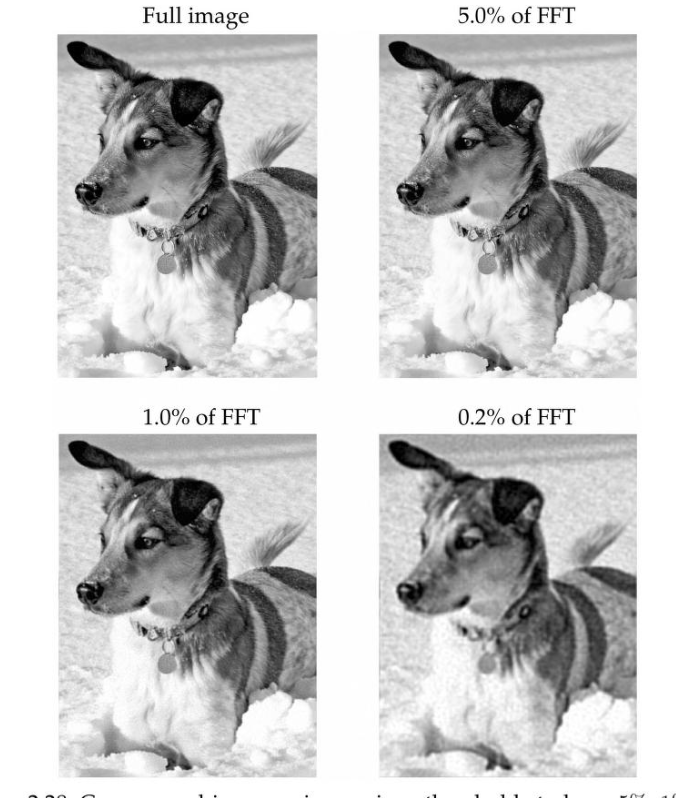
\includegraphics[trim = 0 10 0 0, width=0.5\linewidth, clip]{../pictures/Screenshot 2024-05-22 122030.png}
     \caption{Compressed images} \label{fig:2}
 \end{figure}
\end{frame}
\begin{frame}
	\frametitle{Audio Compression}
	\begin{itemize}
\item The FFT makes audio compression possible.
\item Audio is sampled at 44.1KHz per second.
\item The FFT performs significantly faster than the DFT.
\end{itemize}
\end{frame}
\section{Denoising A Signal}
\begin{frame}
	\frametitle{Denoising A Signal}
	\begin{itemize}
		\item<1-> Generating a signal
		\item<2-> Adding random noise
		\item<3-> Computing The Fast Fourier Transform
		\item<4-> Finding The Power Spectrum Density
		\item<5-> Zero out smaller indices
		\item<6-> Zero out corresponding Fourier coefficients
		\item<7-> Plot And Compare Results 
	\end{itemize}
\end{frame}
\begin{frame}
	\frametitle{The Results}
\begin{figure}[!ht]
    \centering
    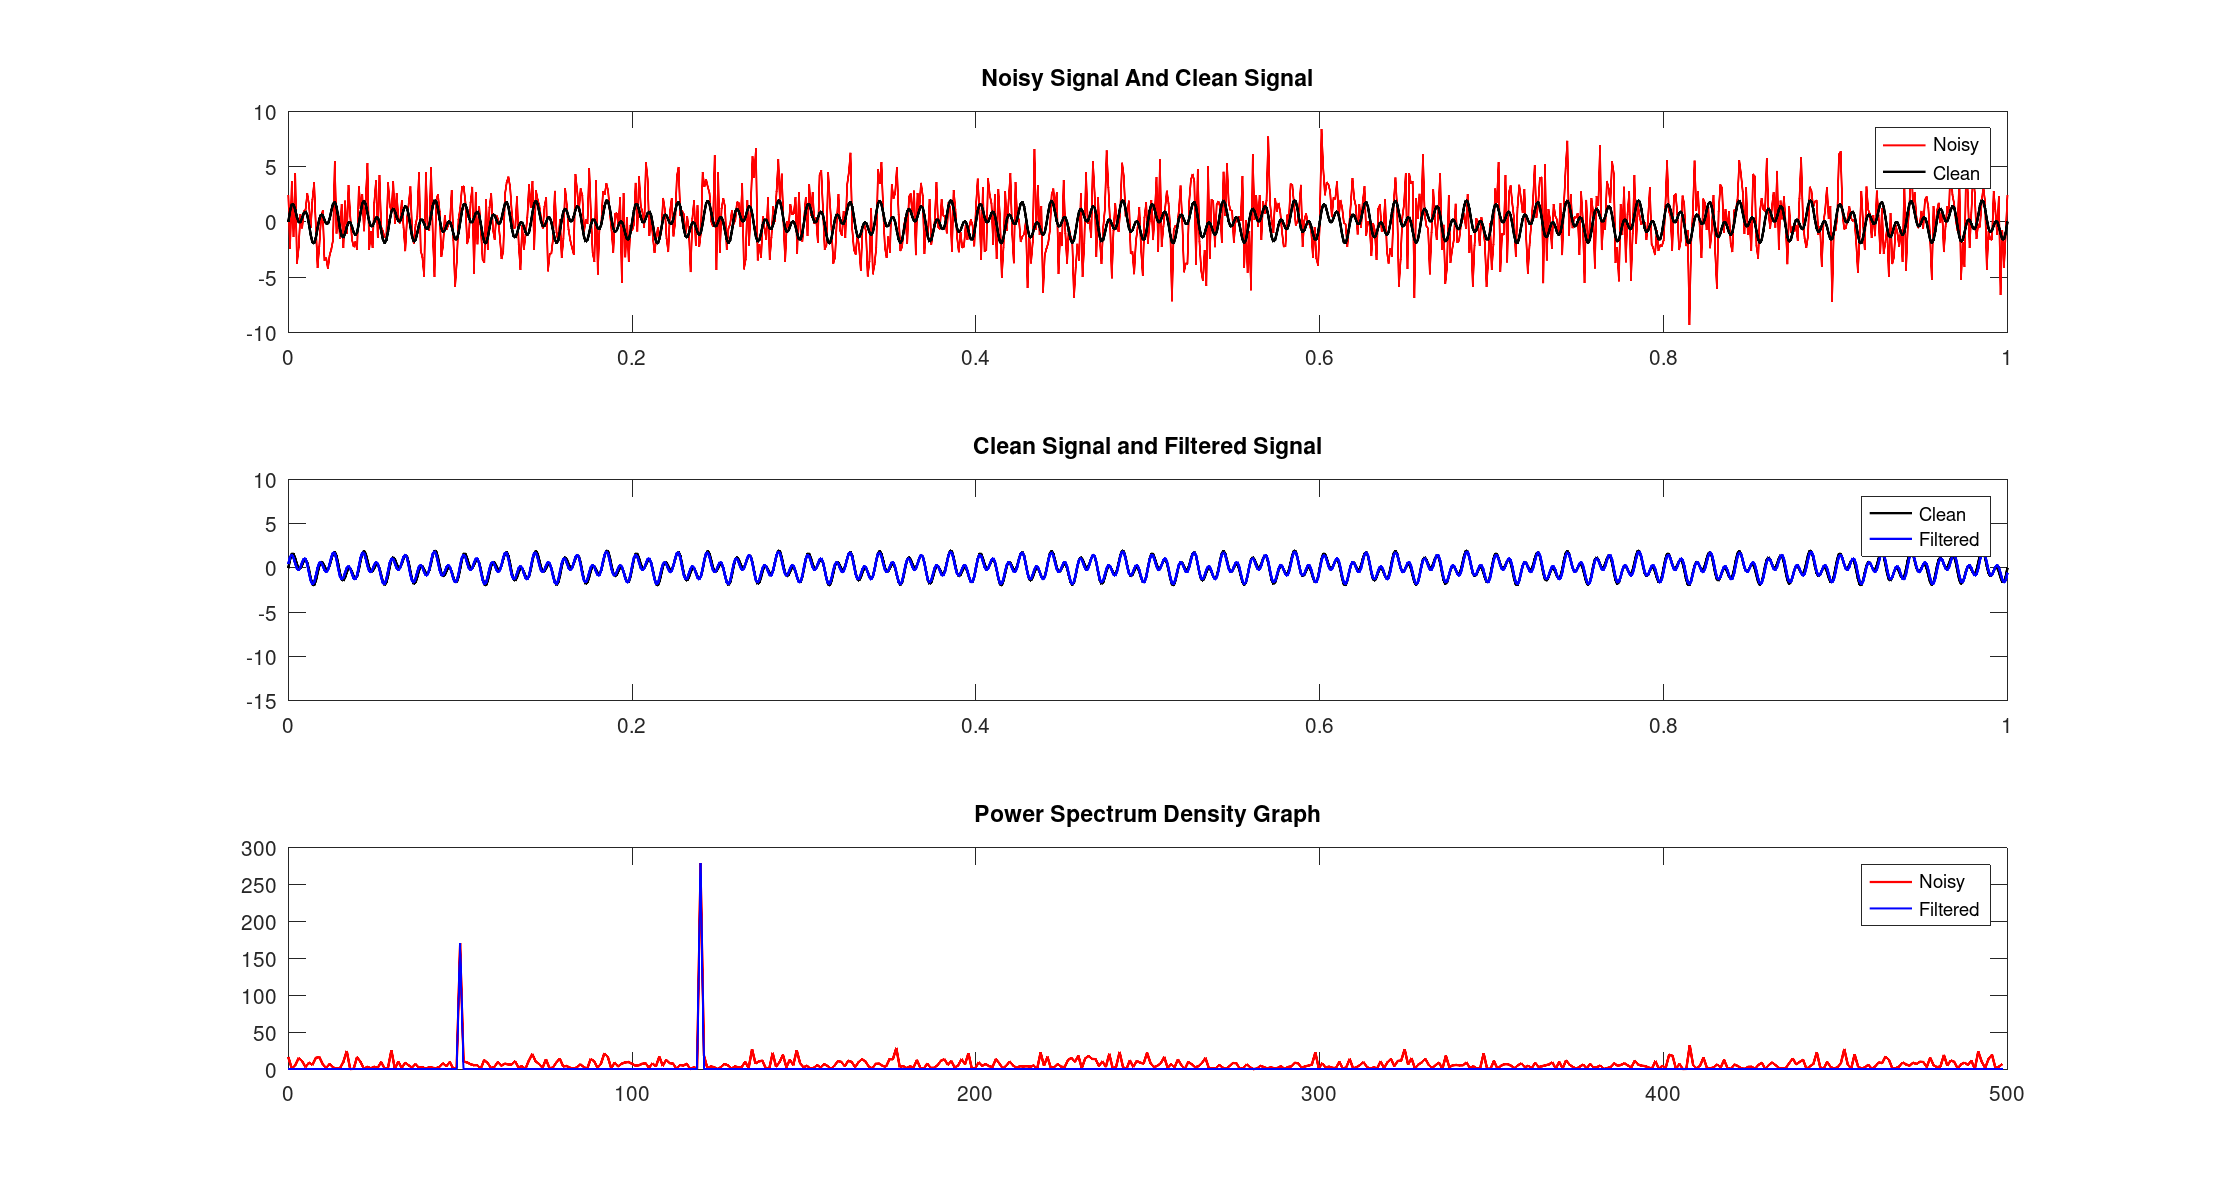
\includegraphics[trim = 0 100 0 50, width=\linewidth,clip]{../plots/denoise.png}
    \caption{(From top to bottom): Plot of noisy signal over clean signal, clean signal over final filtered signal and the power spectrum density graph of noisy signal and filtered signal}
    \label{fig:dft_denoise}
\end{figure}
\end{frame}
\begin{frame}[fragile]
	\frametitle{Code Implementation Of Denoising}
	\begin{lstlisting}
dt = .001;
t = 0:dt:1;
forig = sin(2*pi*50*t) + sin(2*pi*120*t); 
f = forig + 2.5*randn(size(t)); 
n = length(t);
fhat = fft(f,n); 
PSD = fhat.*conj(fhat)/n; 
freq = 1/(dt*n)*(0:n); 
L = 1:floor(n/2); 
%% Use the PSD to filter out noise
indices = PSD>100; 
PSDclean = PSD.*indices; 
fhat = indices.*fhat; 
ffilt = ifft(fhat); 
	\end{lstlisting}
\end{frame}

\begin{frame}
\end{frame}
\begin{frame}
	\frametitle{Thank You}
	``Profound study of nature is the most fertile source of mathematical discoveries." - Joseph Fourier.
\pagebreak
	Noteworthy since, Joseph Fourier discovered the Fourier series while trying tos solve the heat equation
\end{frame}
\end{document}
